\documentclass[
11pt, % The default document font size, options: 10pt, 11pt, 12pt
%oneside, % Two side (alternating margins) for binding by default, uncomment to switch to one side
english, % ngerman for German
singlespacing, % Single line spacing, alternatives: onehalfspacing or doublespacing
%draft, % Uncomment to enable draft mode (no pictures, no links, overfull hboxes indicated)
%nolistspacing, % If the document is onehalfspacing or doublespacing, uncomment this to set spacing in lists to single
%liststotoc, % Uncomment to add the list of figures/tables/etc to the table of contents
%toctotoc, % Uncomment to add the main table of contents to the table of contents
%parskip, % Uncomment to add space between paragraphs
%nohyperref, % Uncomment to not load the hyperref package
headsepline, % Uncomment to get a line under the header
%chapterinoneline, % Uncomment to place the chapter title next to the number on one line
%consistentlayout, % Uncomment to change the layout of the declaration, abstract and acknowledgements pages to match the default layout
]{MastersDoctoralThesis} % The class file specifying the document structure

\usepackage[utf8]{inputenc} % Required for inputting international characters
\usepackage[T1]{fontenc} % Output font encoding for international characters

\usepackage{mathpazo} % Use the Palatino font by default
\usepackage{acro} % Use the acro package for abbreviations

\usepackage[backend=bibtex,style=authoryear,natbib=true]{biblatex} % Use the bibtex backend with the authoryear citation style (which resembles APA)

\addbibresource{literature.bib} % The filename of the bibliography

\usepackage[autostyle=true]{csquotes} % Required to generate language-dependent quotes in the bibliography

%----------------------------------------------------------------------------------------
%	MARGIN SETTINGS
%----------------------------------------------------------------------------------------

\geometry{
	paper=a4paper, % Change to letterpaper for US letter
	inner=2.5cm, % Inner margin
	outer=3.8cm, % Outer margin
	bindingoffset=.5cm, % Binding offset
	top=1.5cm, % Top margin
	bottom=1.5cm, % Bottom margin
	%showframe, % Uncomment to show how the type block is set on the page
}

%----------------------------------------------------------------------------------------
%	THESIS INFORMATION
%----------------------------------------------------------------------------------------

\thesistitle{Speech-Processing-Pipeline to overcome language barriers in real-time communication} % Your thesis title, this is used in the title and abstract, print it elsewhere with \ttitle
\psupervisor{Prof. Dr. Martin Rumpler} % Your primary supervisor's name, this is used in the title page, print it elsewhere with \psupname
\ssupervisor{Prof. Dr. Klaus-Uwe Gollmer} % Your secondary supervisor's name, this is used in the title page, print it elsewhere with \ssupname
\examiner{} % Your examiner's name, this is not currently used anywhere in the template, print it elsewhere with \examname
\degree{Bachelor of Science (B. Sc.)} % Your degree name, this is used in the title page and abstract, print it elsewhere with \degreename
\author{Jason Rietzke} % Your name, this is used in the title page and abstract, print it elsewhere with \authorname
\addresses{} % Your address, this is not currently used anywhere in the template, print it elsewhere with \addressname

\subject{Computer Science} % Your subject area, this is not currently used anywhere in the template, print it elsewhere with \subjectname
\keywords{} % Keywords for your thesis, this is not currently used anywhere in the template, print it elsewhere with \keywordnames
\university{\href{https://umwelt-campus.de}{Trier University of Applied Sciences, Environmental Campus Birkenfeld}} % Your university's name and URL, this is used in the title page and abstract, print it elsewhere with \univname
\department{\href{https://www.umwelt-campus.de/en/study/study-programmes-continuing-education/bachelor/environmental-informatics-and-business-information-systems-bsc}{Environmental Informatics and Business Information Systems}} % Your department's name and URL, this is used in the title page and abstract, print it elsewhere with \deptname
\group{} % Your research group's name and URL, this is used in the title page, print it elsewhere with \groupname
\faculty{Umweltplanung / Umwelttechnik} % Your faculty's name and URL, this is used in the title page and abstract, print it elsewhere with \facname

\AtBeginDocument{
\hypersetup{pdftitle=\ttitle} % Set the PDF's title to your title
\hypersetup{pdfauthor=\authorname} % Set the PDF's author to your name
\hypersetup{pdfkeywords=\keywordnames} % Set the PDF's keywords to your keywords
}


%----------------------------------------------------------------------------------------
%	DEFINE ABBREVIATIONS
%----------------------------------------------------------------------------------------

\DeclareAcronym{voip}{
  short=VoIP,
  long=Voice over Internet Protocol,
}
\DeclareAcronym{ide}{
  short=IDE,
  long=Integrated Development Environment,
}
\DeclareAcronym{api}{
  short=API,
  long=Application Programming Interface,
}
\DeclareAcronym{cli}{
  short=CLI,
  long=Command Line Interface,
}
\DeclareAcronym{http}{
  short=HTTP,
  long=Hypertext Transfer Protocol,
}
\DeclareAcronym{json}{
  short=JSON,
  long=JavaScript Object Notation,
}
\DeclareAcronym{udp}{
  short=UDP,
  long=User Datagram Protocol,
}
\DeclareAcronym{wav}{
  short=WAV,
  long=Waveform Audio File Format,
}
\DeclareAcronym{webm}{
  short=WebM,
  long=Web Media File,
}


\begin{document}

\frontmatter % Use roman page numbering style (i, ii, iii, iv...) for the pre-content pages

\pagestyle{plain} % Default to the plain heading style until the thesis style is called for the body content

%----------------------------------------------------------------------------------------
%	TITLE PAGE
%----------------------------------------------------------------------------------------

\begin{titlepage}
	\begin{center}
		{\huge \bfseries \ttitle\par}\vspace{0.4cm}
		\HRule \\[1.5cm]

		\begin{minipage}[t]{0.4\textwidth}
		\begin{flushleft} \large
		\emph{Author:}\\
		\authorname\\[0.3cm]
		\emph{Semester:}\\
		{9th Semester}\\[0.3cm]
		\emph{Date of Submission:}\\
		{January 9th, 2024}\\[0.3cm]

		\end{flushleft}
		\end{minipage}
		\begin{minipage}[t]{0.5\textwidth}
		\begin{flushright} \large
		\emph{Primary Supervisor:} \\
		\psupname\\[0.3cm]
		\emph{Secondary Supervisor:} \\
		\ssupname\\
		\end{flushright}
		\end{minipage}\\[3cm]
		
		\vfill

		\large\textit{
			A bachelor's thesis submitted in fulfillment of the requirements\\ for the degree of \degreename
		}\\[0.3cm]
		\large\textit{in the}\\[0.4cm]
		\large\textit\deptname\\[0.4cm]
		\large\textit{at the}\\[0.4cm]
		\large\textit\univname\\[0.4cm]
		\large\textit{in cooperation with}\\[0.4cm]
		\large\textit{\href{https://livereader.com/}{LiveReader GmbH}}\\[2cm]

		\vfill
	\end{center}
\end{titlepage}

%----------------------------------------------------------------------------------------
%	DECLARATION PAGE
%----------------------------------------------------------------------------------------

\begin{declaration}
\addchaptertocentry{\authorshipname} % Add the declaration to the table of contents
\noindent I, \authorname, declare that this thesis titled, \enquote{\ttitle} and the work presented in it are written 
by myself and that I did not use any other aids and sources than those indicated. All text passages that have been 
taken verbatim or in spirit from other works are marked as such. The work has not been submitted to any other reviewing 
body in the same or a similar form.
\\

\noindent Date: Oberthal, Germany - January 9th, 2024\\
\rule[0.5em]{25em}{0.5pt}

\noindent Signed:\\
\rule[0.5em]{25em}{0.5pt}\\
\noindent {\authorname}\\

\end{declaration}

\cleardoublepage

%----------------------------------------------------------------------------------------
%	ABSTRACT PAGE
%----------------------------------------------------------------------------------------

\begin{abstract}
\addchaptertocentry{\abstractname}

The primary objective of this bachelor's thesis is to develop a testable prototype for a speech-processing pipeline 
that receives audio streams from various sources and transcribes and translates them in near real-time. The prototype 
facilitates communication between emergency control centers and callers speaking different languages. The focus is on 
utilizing open-source technologies like OpenAI Whisper for speech recognition. The System's functionality revolves 
around processing audio streams, segmenting them into individual messages, and managing them within a session context 
specific to foreign language communication. The prototype is integrated into the Notitia application, leveraging 
existing internal modules for user authentication and data-stream integration to the \ac{voip} provider.

The thesis explores the integration of various open-source technologies. It aims to optimize the processing time of the 
speech-processing pipeline to meet the stringent time constraints that characterize emergencies. The average processing 
time of the pipeline is measured for different numbers of simultaneous audio streams to evaluate the performance and 
conclude a sufficient transcription interval.

This work shows that the speech-processing pipeline meets most requirements and is sufficiently fast to handle multiple 
audio streams simultaneously. It also shows that the pipeline can be built using primarily open-source software and 
commodity hardware. The text translation is the only component not based on an open-source project.

This thesis concludes that the speech-processing pipeline is a viable solution for emergency call centers to overcome 
language barriers in real-time communication. It can provide near real-time transcription and translation of spoken 
content and can be deployed on-premise to ensure reliability in emergencies.

\end{abstract}

%----------------------------------------------------------------------------------------
%	LIST OF CONTENTS/FIGURES/TABLES PAGES
%----------------------------------------------------------------------------------------

\tableofcontents % Prints the main table of contents

\listoffigures % Prints the list of figures

\listoftables % Prints the list of tables

%----------------------------------------------------------------------------------------
%	THESIS CONTENT - CHAPTERS
%----------------------------------------------------------------------------------------

\mainmatter % Begin numeric (1,2,3...) page numbering

\pagestyle{thesis} % Return the page headers back to the "thesis" style

% Include the chapters of the thesis as separate files from the Chapters folder
% Uncomment the lines as you write the chapters

\chapter{Introduction}

\label{Chapter1}

%----------------------------------------------------------------------------------------

% Define some commands to keep the formatting separated from the content 
\newcommand{\keyword}[1]{\textbf{#1}}
\newcommand{\tabhead}[1]{\textbf{#1}}
\newcommand{\code}[1]{\texttt{#1}}
\newcommand{\file}[1]{\texttt{\bfseries#1}}
\newcommand{\option}[1]{\texttt{\itshape#1}}

%----------------------------------------------------------------------------------------

\section{Background \& Motivation}

% This work is conducted in the context of the Notitia Suite of the LiveReader GmbH, within the SPELL research project. 
% The SPELL research projects aims to improve the software of critical infrastructures, such as emergency control 
% centers. In this context the Notitia Suite serves the prupose of a interface for the emergency calltaker to dispatch 
% the emergency services. \\
% \\
% An important part of dispatching the proper resources is to understand the needs of the emergency caller. 
% This is especially difficult when the caller and the calltaker do not speak the same language and important details 
% can not be conveyed properly. \\
% \\
% This work aims to develop a speech-processing pipeline that can be integrated into the Notitia Suite to allow for 
% communication between the caller and the calltaker speaking foreign languages. The pipeline itself is able to work 
% stand alone and can be integrated into other applications but does not have to be. \\
% This work will focus on the development of the speech-processing pipeline from here on and won't go into detail 
% regarding intigration into the Notitia Suite or any other application that may use it as a service.

Effective communication is critical in emergency services, where timely and accurate information is vital to 
saving lives. The Notitia application, within the context of the SPELL research project, aims to establish a 
communication framework between emergency control centers and callers. The project envisions a seamless integration of 
a speech-processing pipeline to transcribe and translate audio streams in real-time, addressing the language barriers 
that often impede clear communication during emergencies.

The SPELL research project recognizes the importance of near real-time transcription and translation services in empowering emergency control centers—existing technologies present challenges that need innovative solutions. 
Many systems designed for continuous audio streams are cloud-based, introducing concerns regarding reliability, 
latency, and request priority—critical factors in emergency services. The proposed solution aims to 
overcome these challenges by leveraging open-source technologies and building a testable prototype that can be deployed 
on-premise, ensuring reliability in time-sensitive scenarios.

%----------------------------------------------------------------------------------------

\section{Problem Statement}

% Despite the advancements in speech processing, existing solutions for transcription and translation in continuous audio 
% streams often fall short of meeting the specific demands of emergency call centers. Cloud-based systems, while widely 
% available, pose risks related to their reliability and latency, which are critical considerations in the context of 
% emergency response. The inability to seamlessly integrate features from different providers further hinders the 
% optimization of the transcription and translation process.\\
% \\
% The challenge, therefore, is to develop a speech-processing pipeline that not only addresses the language barriers in 
% emergency communication but also meets the stringent requirements of reliability, low latency, and on-premise 
% deployment. The integration of OpenAI Whisper, DeepL, and PiperTTS as foundational technologies sets the stage for a 
% comprehensive solution, yet the task is to weave these components into a coherent system tailored for emergency 
% services.

Despite the rapid advancements in speech processing technologies, the unique demands of emergency call centers pose 
significant challenges that current solutions need help to overcome. The SPELL research project identifies a crucial gap 
in systems designed for continuous audio streams. While cloud-based platforms offer convenience and 
scalability, they introduce a host of concerns when applied to the critical infrastructure of emergency services. 
Issues such as reliability, latency, and request prioritization become magnified in time-sensitive scenarios, 
jeopardizing the effectiveness of emergency responses.

The reliance on cloud solutions also restricts the flexibility to deploy services on-premise, a key consideration for 
maintaining the operational integrity of emergency control centers. Moreover, the homogeneous nature of many 
speech-processing systems impedes the seamless integration of features from diverse providers. This limitation prevents 
emergency services from harnessing the full spectrum of capabilities offered by various tools, hindering the 
optimization of transcription and translation processes.

In essence, the challenge is not just about overcoming language barriers; it is about tailoring a solution that aligns 
with the unique requirements of emergency communication. The proposed speech-processing pipeline must be a fusion of 
innovation and practicality, addressing linguistic diversity and the critical need for reliability, low 
latency, and the ability to operate on-premise.

Therefore, the problem is multifaceted: How can a speech processing pipeline be meticulously crafted to 
transcend the limitations of current technologies, providing a reliable, low-latency, and on-premise solution for 
emergency call centers? This challenge necessitates an exploration of open-source technologies, strategic integration 
of proven components like OpenAI Whisper and DeepL, and the development of a tailored prototype, all within the 
stringent time constraints that characterize emergencies. The task is to navigate the intricacies of emergency 
communication, ensuring that the proposed solution becomes an indispensable tool for effective and timely response in 
the face of linguistic diversity.


%----------------------------------------------------------------------------------------

\section{Objectives \& Scope}

The primary objective of this bachelor's thesis is to develop a testable prototype for a speech-processing pipeline 
within the Notitia application. This prototype aims to transcribe and translate audio streams in near real-time, 
facilitating communication between emergency control centers and callers speaking different languages. The focus is on 
utilizing existing open-source technologies, such as OpenAI Whisper for speech recognition, DeepL for translation, and 
PiperTTS for speech synthesis.

The scope encompasses the integration of the speech-processing pipeline into the Notitia application, leveraging 
existing internal modules for user authentication and data-stream integration to the Voice over IP provider. The 
system's functionality revolves around processing audio streams, segmenting them into individual messages, and managing 
them within a session context specific to foreign language communication.

%----------------------------------------------------------------------------------------

\section{Research Questions \& Methodology}

\subsection{Research Questions}

How can a speech processing pipeline, predominantly built upon open-source software, be harnessed to facilitate near 
real-time transcription and translation of spoken content to overcome language barriers in the context of an emergency 
call center?

\subsection{Methodology}

The research methodology involves the development of a testable prototype with a focus on minimizing processing time. 
The integration of OpenAI Whisper, DeepL, and PiperTTS will be explored to optimize the transcription and translation 
process. The system will utilize existing internal modules for user authentication and data-stream integration, with a 
data stream transferring audio in WAV format. The research emphasizes on-premise deployment for reliability in 
emergency scenarios.

In the subsequent chapters, we delve into the technical details of the speech-processing pipeline, its integration into 
Notitia, and the evaluation of its performance in the critical context of emergency communication.


\chapter{Concept}

\label{Concept}

The concept chapter of this work gives a brief overview of what components are doing and how they are related. 
A detailed look at each component and its inner workings comes in the following chapters of this work.

%----------------------------------------------------------------------------------------

\section{Workflow Diagram}

\begin{figure}[ht]
	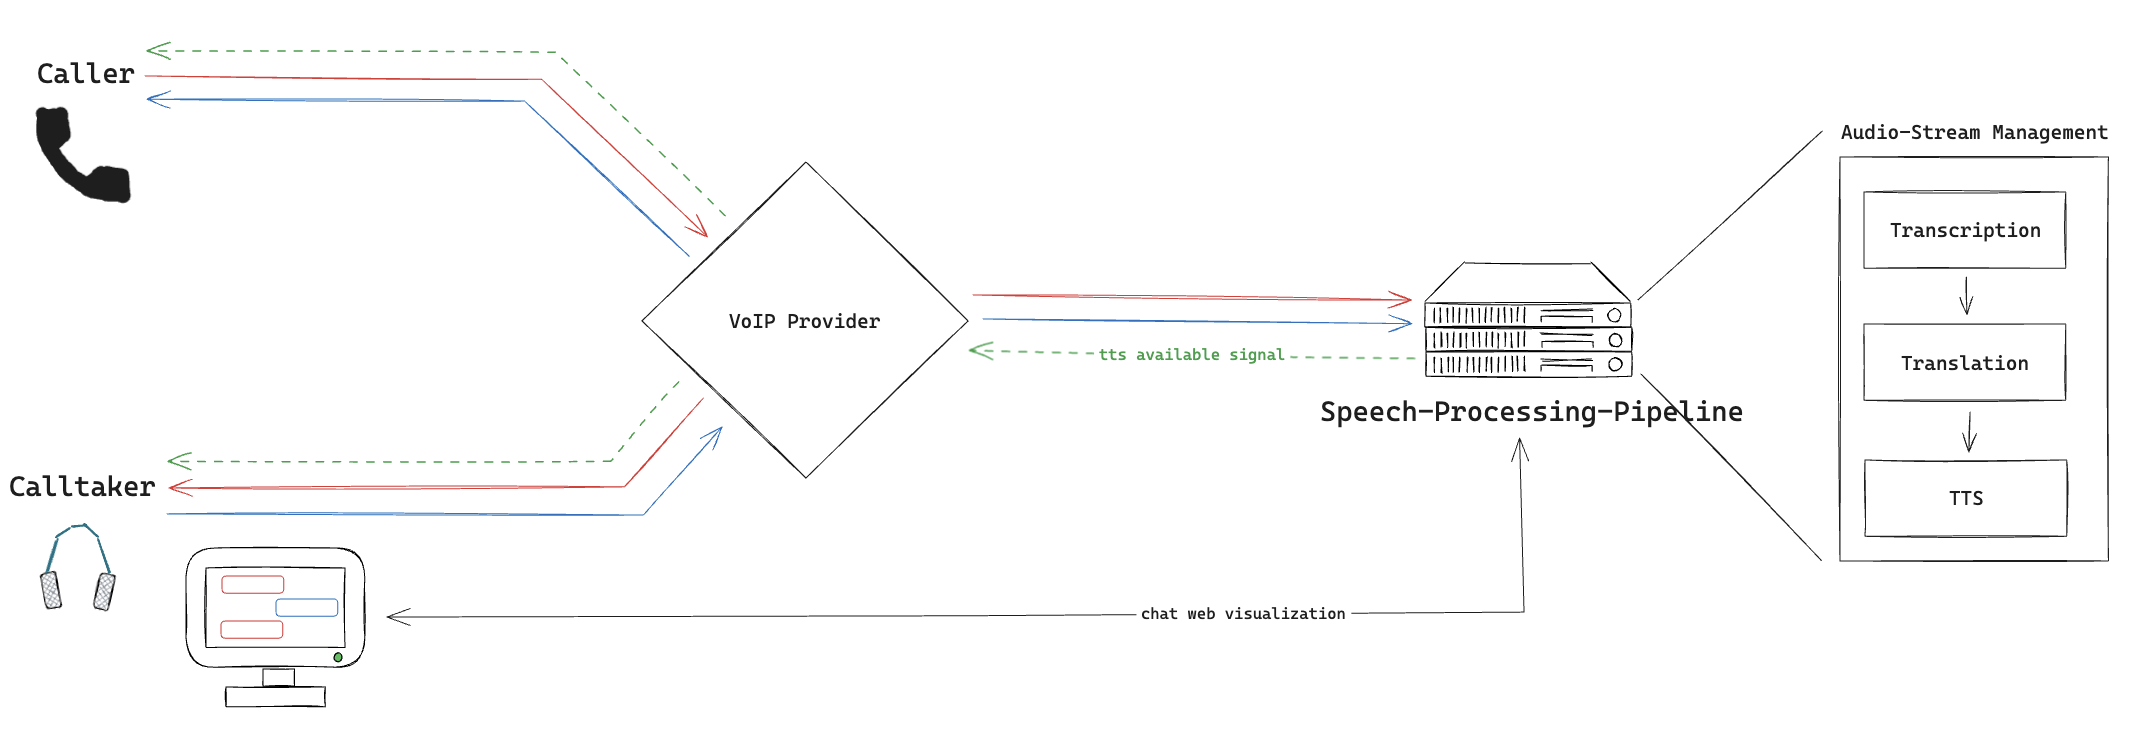
\includegraphics[width=\textwidth]{Figures/data-flow-chart.png}
	\caption{Workflow Diagram}
	\label{fig:workflowDiagram}
\end{figure}

Figure \ref{fig:workflowDiagram} shows a high-level overview of the System's workflow. It shows the phone call between 
the emergency caller and the call-taker. It is routed through the \ac{voip} provider, which forwards the audio stream to 
the speech-processing pipeline server. The server then processes the audio stream by transcribing, translating, and 
synthesizing it. The resulting tts signal gets sent back to the \ac{voip} provider, who plays it back to the caller and 
call-taker, respectively.

The graphic also shows the chat visualization in the web browser. This visualization is optional and can only be used 
by the call-taker in the displayed scenario.

%----------------------------------------------------------------------------------------

\section{Audio Input}

The flexibility of the System allows for various audio input options. This work will cover two of the most important 
ones. The two most critical audio sources are recordings by web browsers and audio input provided by \ac{voip} 
communication systems. This module is described in detail in Chapter \ref{AudioDataReception}.

\subsection{Web Browser Audio}

Within the context of this work, the focus lies on integrating Chromium-based web browsers. The Web MediaRecorder API 
provides the audio input. The API requests access to the microphone and allows for recording audio streams. 
The audio stream gets sent to the server as \ac{webm}-encoded data chunks of about 200ms. The server then concatenates 
the chunks and converts the audio stream to \ac{wav} format. The conversion utilizes FFmpeg, a \ac{cli} tool for 
manipulating audio and video files. The speech-processing pipeline then processes the resulting \ac{wav} file.

\subsection{Voice-over-IP Audio}

To get access to \ac{voip} audio data, a third party gets access to the \ac{api} and forwards the data stream to the 
system. This stream comes via \ac{udp} and contains 20ms of uncompressed \ac{wav} audio data for each chunk.
Each chunk carries an identifiable tag that allows the system to map the audio data against a user.
These chunks get concatenated to be processed by the speech-processing pipeline.

%----------------------------------------------------------------------------------------

\section{Speech Processing}

The speech processing component mainly comprises a microservice wrapping OpenAIs Whisper project. It receives slices of 
the audio stream, various in length, and transcribes them into text. The transcription is then analyzed, and if there 
is no change in content for more than two iterations, it finalizes the pending message. Any new content will cause the 
creation of a new message object, and the process will start over. This module is described in detail in Chapter 
\ref{SpeechProcessing}.

The speech-processing pipeline utilizes Whisper to determine the spoken language as well. It returns the most likely 
language used in the audio file. Alongside the integrated voice-activation feature to filter out sections that do not 
contain spoken content, Whisper is a very versatile tool.

After a message is determined to have ended, the system utilizes DeepL to translate the message into any foreign 
language spoken within the same session, described in detail in Chapter \ref{SessionHandlingAndMessageTranslation}.

%----------------------------------------------------------------------------------------

\section{Session Handling}

After creating a new session with its corresponding ID, users can join it by connecting to it with an audio stream. 
Each audio stream is related to a known Notitia User account or gets a temporary user object. In the latter case, the 
user will not be able to be identified as the same one if the audio connection drops and gets reconnected. 
This module is described in detail in Chapter \ref{SessionHandlingAndMessageTranslation}.

The session object holds various data about the connected audio streams, their users, and the determined spoken 
languages of each one. This data leads to generating the necessary translations of a message. A session is also 
responsible for broadcasting the information about generated audio files to the appropriate receivers.

It is possible to connect any number of users to one singular session. However, within this work, a two-user session is 
most common since it represents the use case of an emergency caller and call-taker.

%----------------------------------------------------------------------------------------

\section{Audio Output}

After the translated text is available, the system can synthesize an audio file. The audio file gets created 
using PiperTTS, an open-source text-to-speech library. The library supports multiple languages and voices. The 
resulting audio file gets sent back to users via the appropriate audio output channel. This procedure is different 
depending on the audio input channel. This module is described in detail in Chapter 
\ref{SpeechSynthesisAndAudioDataTransmission}.

\subsection{Web Browser Audio}

If the user connects via a browser audio stream, the system sends a WebSocket message to the client to notify it about 
the existence of a newly synthesized file. The web client uses the transmitted ID property to download the audio 
\ac{wav} file and uses the Web Audio \ac{api} to play it back.

\subsection{Voice-over-IP Audio}

If the user connects via a \ac{voip} provider, the system sends a \ac{udp} message to the provider via a previously 
configured backchannel port. The message contains the ID of the audio file, and the \ac{voip} provider uses the ID to 
download the audio \ac{wav} file and plays it back into the audio stream of the phone call.

\chapter{Audio Data Reception}

\label{AudioDataReception}

The system is versatile and is capable of handling a wide variety of input audio data streams. The scope of this work, 
however, focuses on the reception of web browser audio input and Voice over IP audio input.

%----------------------------------------------------------------------------------------

\section{Audio Connection}

Any specific audio reception point returns the generic AudioConnection class and allows the rest of the system to 
handle every audio connection the same. 
It contains data about its assigned session, the user it belongs to, and the audio input channel it uses.

It also provides an event-based interface so the rest of the system can listen to specific events and react  
accordingly. The available events are the "close" event, which gets fired when the audio connection gets closed, and 
the "message" event, which gets fired when new data from the audio stream is available.

This architecture provides a unified interface for the entire system to handle audio streams and their data.

\begin{verbatim}
// audioConnection.ts
export type EventType = "message" | "close";
export class AudioConnection {
    get closed() {}
    readonly id: string;
    readonly sessionId: string;
    readonly userId: string;
    readonly userName: string | undefined;
    readonly rtpRegisterEntry: RTPRegisterEntry | undefined;

    constructor(
        id: string,
        sessionId: string,
        userId?: string,
        userName?: string,
        rtpRegisterEntry?: RTPRegisterEntry,
    ) {}

    emitMessage(message: Buffer) {}
    close() {}
    on(type: EventType, cb: (arg: Buffer | void) => void): number {}
    off(id: number) {}
}
\end{verbatim}

%----------------------------------------------------------------------------------------

\section{Web Browser Audio}

The web browser audio input is the most straightforward audio input channel. It is based on WebSockets and
uses the WebSocket API to receive audio data from the client. The client uses the MediaRecorder API to capture the 
audio data from the microphone and sends it to the server via the WebSocket connection.

\subsection{Transmitter}

The web browser joins a WebSocket connection to the server and sends the audio data as a binary message to the server. 
It requests access to the microphone and uses the MediaRecorder API to capture the audio data. 
The audio data is requested in chunks of approximately 200ms and sent to the server as a WebM-encoded binary message.

\subsection{Receiver}

On the other hand, the receiving WebSocket Server takes the chunk, converts the data into a WAV file format by 
utilizing FFMPEG, and fires the appropriate AudioConnection "message" event to inform all listeners about the new data.


\chapter{Speech Processing}

\label{SpeechProcessing}

The speech-processing component mainly comprises a microservice wrapping OpenAIs Whisper project and the management 
that utilizes this component to process audio streams. It receives slices of the audio stream, various in length, and
transcribes them into text.

Since Whisper cannot process audio streams directly but can only complete audio files, this service is required to 
build the basis to transcribe slices of the audio stream continuously. The speech-processing pipeline uses this service 
to support audio streams and near real-time transcription.

%----------------------------------------------------------------------------------------

\section{Microservice Wrapper}

The speech-processing pipeline contains a microservice for processing audio streams with OpenAIs Whisper. It receives 
transcription requests via an \ac{http} \ac{api} and returns the resulting \ac{json} information about the audio file.

\subsection{Faster Whisper}

Since the system's hardware uses Nvidia graphics cards, the microservice uses a GPU-accelerated version of Whisper 
called Faster Whisper, \cite{fasterwhisper2023github}. It brings CUDA support to allow for GPU-accelerated processing 
of audio files when dealing with Nvidia graphics cards. The microservice checks for the availability of CUDA support on 
startup and falls back to the CPU version if it is unavailable.

Since the interface for Faster Whisper is only available in the Python programming language, but the interfacing 
service is preferred to be developed in Node.js, the Whisper access is implemented by building a \ac{cli} interface 
that calls all necessary operations of Faster Whisper. This design decision allows the developer to test the whisper 
interface independently since it can run as a terminal application.

The Node.js interface for the microservice itself spawns a child process that runs this application and communicates 
with it over the standard input/output.

\subsection{Service Pool}

The versatility of this design pattern made another improvement very easy to implement. Since the capabilities of 
different graphics cards are various, and one audio file processing job might not utilize the full potential of the 
hardware in question, it makes sense to provide a service pool with a configurable amount of transcription workers 
available. One transcription worker would be one instance of the previously explained \ac{cli} tool.

Due to the chosen design, this improvement is natural by holding a ServicePool with numerous worker instances. When 
requesting a job, the pool uses the next available worker instance.

\subsection{Interface}

The \ac{http} interface of the microservice is straightforward. It provides a single endpoint for transcribing audio 
files and returns the resulting \ac{json} information about the audio file. The endpoint is available under the root 
path of the microservice and expects a POST request with the audio file as the body of the request. The audio file has 
to be in a \ac{wav} format and encoded as base64. There is also an optional query parameter to specify the language of 
the audio content. The microservice returns the resulting \ac{json} information about the audio file.

\subsection{Whisper Model Sizes}

The OpenAI Whisper project provides multiple models with different sizes, accuracy, and performance. The microservice 
uses the most powerful model available, "large-v2," by default since it provides the best accuracy, which is crucial 
for the System. However, the microservice allows the specification of a different model size on the environment 
variable level. This allows the developer to use a smaller model size for testing purposes or a larger one for 
production.

An extensive list of available models can be found in the research paper of OpenAI \cite{radford2022robust}. 
The provided overview of the different model sizes is shown in Table \ref{tab:whisper-model-sizes} and refers to the 
GitHub repository of the project \cite{whisper2022github}.

\begin{table}[ht]
	\centering
	\begin{tabular}{|l|l|l|l|l|}
		\hline
		Size & Parameters & Multilanguage Model & VRAM & Rel. speed \\
		\hline
		tiny & 39 M & tiny & $\sim$1 GB & $\sim$32x \\
		base & 74 M & base & $\sim$1 GB & $\sim$16x \\
		small & 244 M & small & $\sim$2 GB & $\sim$6x \\
		medium & 769 M & medium & $\sim$5 GB & $\sim$2x \\
		large & 1550 M & large & $\sim$10 GB & 1x \\
		\hline
	\end{tabular}
	\caption{Whisper Model Sizes}
	\label{tab:whisper-model-sizes}
\end{table}

%----------------------------------------------------------------------------------------

\section{Language Detection}

If Whisper has no information about the language of the audio file, it determines a list of possible languages. The 
audio file transcription gets generated in the language with the highest probability. The speech-processing pipeline 
also uses this integrated language detection to determine the language of the audio stream.

Since this is not always accurate, especially with short audio files, the speech-processing pipeline brings additional 
safeguards to reduce the chance of misinterpreted audio files.

Suppose there is no previously known language for the user that sends the audio stream. In that case, the transcription 
microservice will not get any assumption about the language and, therefore, determine it by itself. This language will 
be returned and saved as the user's language for future audio streams.

Since this assumption can be false, or the user might switch to another language, the speech-processing pipeline 
assumes the previous language as long as a message has less than five words. From this point on, language detection 
will reactivate again to determine the language of the audio stream. This safeguard reduces the chance of 
misinterpreted audio files since the user will most likely not switch the language of the audio stream in the middle 
of the conversation. Concise messages are the most vulnerable to language detection errors, and this protection 
reduces these.

%----------------------------------------------------------------------------------------

\section{Transcription}

The transcription response of the microservice contains a list of all recognized words and their probability. The 
speech-processing pipeline uses this to create the transcription of the audio stream. Words with a low probability are 
uncertain and can be highlighted to the user in the user interface.

The speech-processing pipeline requests a transcription of the audio stream every 1500ms by default. If the 
transcription has not changed since the previous request, the message will be assumed to be complete, and the recorded 
audio data will be cut off to start a new buffer for the following message. This design decision allows the system to 
efficiently handle multiple messages in a row without interrupting the audio stream.

Silence will cause such a cut since the audio file did not contain any additional spoken content, thus causing the 
transcription to stay the same. After starting to speak, the audio buffer contains spoken content again, and the 
transcription will contain new information. This new transcription input causes the creation of a new message, which 
will be pending until the transcription does not change for about 1500ms again.

The reason for the transcription interval of 1500ms is documented in detail in the Evaluation chapter \ref{Evaluation}.

\chapter{Session Handling and Message Translation}

\label{SessionHandlingAndMessageTranslation}

The session handling and message translation components are responsible for managing the interaction between the 
different session participants and translating the messages between the different languages if necessary.


\chapter{Speech Synthesis and Audio Data Transmission}

\label{SpeechSynthesisAndAudioDataTransmission}

Speech synthesis and transmitting the resulting audio data to the proper users is crucial for the System to work. The 
following components are responsible for this task. Especially for users only connected via Voice over IP, this is the 
only way to provide them with the translated message.

%----------------------------------------------------------------------------------------

\section{Speech Synthesis}

The System uses PiperTTS, an open-source text-to-speech library, to synthesize spoken audio from text. It supports 
multiple languages and voices and allows the System to create audio files in any language with a voice model.

The System uses PiperTTS to create audio files from the translated messages. The audio files are stored in the 
filesystem and available via a unique ID. The ID gets returned to the session handling component, which uses it to send 
the audio file to the appropriate users.

\subsection{TTS Microservice}

Like the transcription microservice, the speech synthesis microservice wraps the PiperTTS CLI interface and 
provides a convenient HTTP API interface to the rest of the System. The service spawns a child process that runs the 
PiperTTS CLI application and awaits the generation of the audio file. It then returns the audio file as an HTTP response 
encoded as audio/wav.

The HTTP interface of the microservice is straightforward. It provides a single endpoint for synthesizing audio files 
and returns the resulting audio file. The endpoint is available under the root path of the microservice and expects a 
POST request with the text to synthesize as the body of the request. There is one required query parameter to specify 
the language of the audio content. Additionally, there are optional query parameters to specify the preferred country, 
gender, or a specific voice model. The microservice returns the resulting audio file.

\begin{verbatim}
POST / HTTP/1.1
Content-Type: text/plain
Content-Length: 28
Accept: audio/wav

Hello World, this is a test.

\end{verbatim}

\subsection{Audio Generation}

Since PiperTTS utilizes the entire CPU by splitting the audio generation into as many threads as there are CPU cores, 
the System can utilize the hardware's full potential without creating a service pool like the transcription 
microservice.

The generated audio file is in the WAV format and encoded as audio/wav. The System stores the audio file in the 
filesystem. It returns the ID of the audio file to the session handling component—the session handling component uses 
the ID to send the audio file to the appropriate users. 

%----------------------------------------------------------------------------------------

\section{Audio Data Transmission}

After the audio file is available, the System needs to send it to the appropriate users. This procedure is different 
depending on the audio input channel. The System uses WebSockets to send the audio file to users connected via a web 
browser. For users connected via Voice over IP, the System uses a UDP backchannel to send the audio file to the VoIP 
provider.

\subsection{Web Browser Audio}

If the user connects via a browser audio stream, the System sends a WebSocket message to the client to notify it about 
the existence of a newly synthesized file. The web client uses the transmitted ID property to download the audio WAV 
file and uses the Web Audio API to play it back.

The WebSocket message contains the ID of the audio file as well as data about the nature of the synthesized audio file. 
The web client uses this information to determine the correct way to play back the audio file. The System sends the 
following WebSocket message to the client.

\begin{verbatim}
{
    "type": "tts",
    "audioId": "1c4e0c77-f3d9-5ba5-bc88-c2177926514d",
    "playbackType": "translation"
}
\end{verbatim}

The "type" property allows the use of one single WebSocket connection for all kinds of messages and helps the client 
determine the correct way to handle the message. In this case, it is a text-to-speech event. The "audioId" property 
contains the ID of the audio file. The "playbackType" property contains the type of the audio file. In this case, it is 
a translation of a message sent by another user. It can also be assigned to the value "translation-playback." The 
"translation-playback" value is used to play back the translation of the user's message.

With this design decision, the User Interface can easily support features to play back the translations in different 
volume levels or even allow client-side configuration to turn off the playback of specific translations altogether.

\subsection{Voice over IP Audio}

If the user connects via a VoIP provider, the System sends a UDP message to the provider via a previously configured 
backchannel port. The message contains the ID of the audio file, and the VoIP provider uses the ID to download the 
audio WAV file and plays it back into the audio stream of the phone call. 

The UDP message contains only the ID of the audio file. The VoIP provider uses the ID to download the audio file and 
play it back to the user. The System sends the following UDP message to the VoIP provider. 

\begin{verbatim}
WaveFile:30ea2c43-bbdc-5db6-8d46-78ddbc2b1b72
\end{verbatim}

\chapter{Evaluation}

\label{Evaluation}

This chapter evaluates the System's capabilities and compares them to the requirements defined in Chapter 
\ref{Introduction}. It analyzes the System's performance and its ability to handle multiple audio streams 
simultaneously.

%----------------------------------------------------------------------------------------

\section{Streaming Capability \& Transcription Interval}

Since Whisper does not support real-time audio transcription, the System had to be designed to handle audio streams 
and utilize Whisper to transcribe slices of the audio stream. By implementing this feature, the System 
enhances the capabilities of Whisper and allows it to transcribe audio streams in near real-time.

The System slices the stream into chunks and transcribes them individually. The frequency of the transcription - 
and therefore the size of the chunks - is configurable using the "TranscriptionInterval" environment variable.

The following analysis compares the System's required transcription processing time with various amounts of 
simultaneously processed audio streams. The System runs on a machine with two Nvidia GeForce RTX 4070 graphics cards. 

The following table shows the average processing times for one, two, four, and eight simultaneous audio streams.

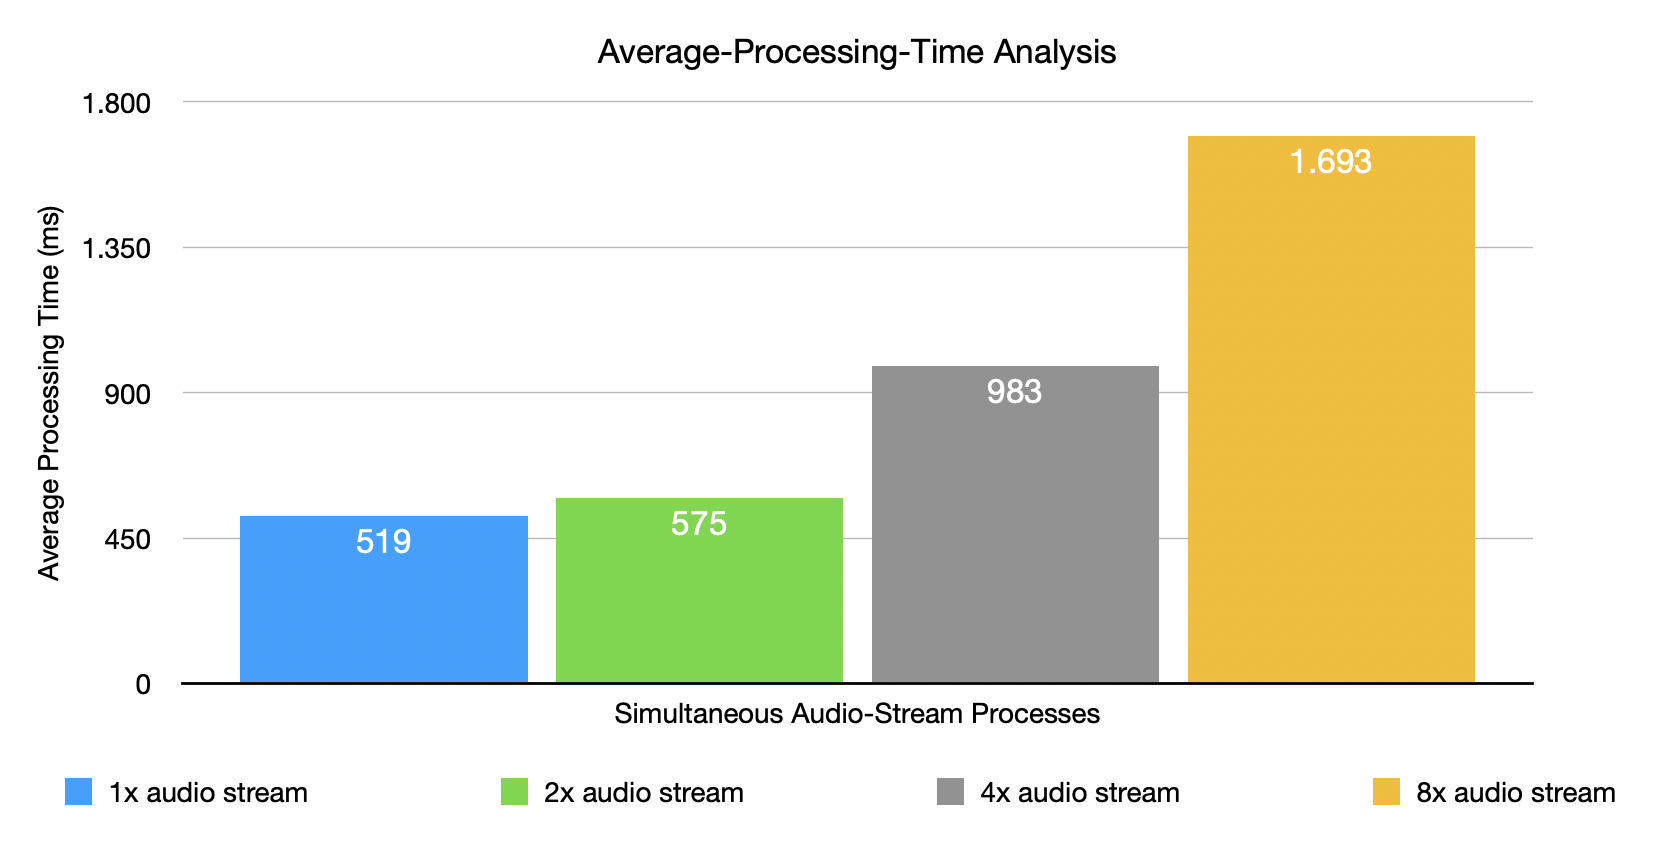
\includegraphics[scale=0.45]{Figures/avg-processing-times.png}

The diagram shows that the average processing time for one audio stream is 519 milliseconds. This would suggest that a 
transcription interval of about 520 milliseconds would be optimal for a hardware configuration like this. 

However, the diagram also reveals that the average processing time for two audio streams is 575 milliseconds. This 
seems unintuitive at first glance, but it is because the System utilizes a hardware setup with two graphics cards. 
The System can process two audio streams simultaneously, each on a separate graphics card. This results in a minor 
processing time increase for each audio stream since the System only shares CPU and data transmission resources between 
the two audio streams - not the GPU performing the transcription.

Looking at the average processing time for four simultaneous audio streams, we can see that it is 983 milliseconds. 
This significantly increases compared to the average processing time for two audio streams. This is because the System 
has to share the GPU resources between four audio streams - two on each graphics card. This results in a significant 
increase in processing time for each audio stream.

As shown in the last column of the diagram above, the average processing time for eight simultaneous audio streams is 
1,693 milliseconds. This significantly increases compared to the average processing time for four audio streams. 
This is because the System has to share the GPU resources between eight audio streams - four on each graphics card. 

\subsection{GPU Utilization}

The observation that the processing time increases are not doubled when the number of audio streams is doubled suggests 
that the utilization of the GPU is improved by running multiple audio transcriptions simultaneously. The GPU is only 
partially utilized when processing a single audio stream. A second, third, or fourth audio stream can utilize more GPU 
resources even though the processing time increases overall.

\subsection{1500ms Transcription Interval}

To ensure the System can handle multiple audio streams simultaneously, it uses a transcription interval of 1500 
milliseconds by default. This transcription interval is configurable using the "TranscriptionInterval" environment 
variable. The transcription interval is the time between two transcriptions of the same audio stream.

1500 milliseconds is a good default value for the transcription interval because it allows the System to support up to 
eight simultaneous audio streams on a machine with two Nvidia GeForce RTX 4070 graphics cards. When all eight audio 
streams are active, the System has a processing time more significant than the transcription interval. To prevent this, 
the System awaits the results of the previous transcription before starting a new one for the same audio stream. This 
ensures that the System can handle up to eight simultaneous audio streams without requesting more resources than are 
available.

\chapter{Conclusion}

\label{Conclusion}

This chapter summarizes the System's capabilities and compares them to the requirements defined in Chapter 
\ref{Introduction}. It also discusses the System's limitations and potential future work.

%----------------------------------------------------------------------------------------

\section{Summary}

This thesis aimed to develop a System that allows users to communicate with each other in foreign languages in near 
real-time. The System should be able to handle multiple audio streams simultaneously and detect the spoken language 
automatically. It should also be able to translate the audio content into the user's preferred language and provide the 
translated text and audio to the user. Furthermore, the System should be built using open-source software and be able 
to run on commodity hardware.

The System developed in this thesis can handle audio streams from web browsers and provides an interface for Voice over 
IP providers to send a UDP audio stream to be processed, aiming to integrate with VoIP providers. The pipeline takes 
the various audio sources, transforms them internally into the same format, and handles them the same way from that 
point on.

The near real-time transcription of the audio streams is achieved by utilizing the open-source OpenAI Whisper project. 
The System enhances Whisper's capabilities by enabling it to transcribe audio streams instead of final audio files. 
This reaches the goal of streaming support and near real-time transcription.

Automatic language detection is achieved by utilizing the same Whisper service. It has a very capable language 
detection feature that can detect the spoken language of an audio stream with high accuracy.

The System uses the open-source PiperTTS project to synthesize spoken audio from text. It allows the System to 
synthesize audio files with various voices in different languages. The System uses PiperTTS to synthesize audio files 
from the translated messages and stores them in the filesystem. Implementing this feature reaches the goal of speech 
synthesis based on open-source software.

The only external proprietary component the speech-processing pipeline uses is the DeepL translation API to translate 
the transcription results into the required languages within a session. This is the only component that is not 
open-source since the quality and versatility of open-source translation services do not meet expectations.

%----------------------------------------------------------------------------------------

\section{Potential Future Work}
Even though the developed speech-processing pipeline meets most requirements, there is still room for improvement. 
The following sections discuss potential future work.

\subsection{Open-Source Translation Service}

The System uses the DeepL translation service to translate the transcription results into the required languages. 
DeepL is a commercial translation service that provides a high-quality translation API. However, the versatility of the 
System design allows for the future replacement of the DeepL translation service with an open-source solution. 

Since new AI models are continuously being developed, open-source translation services may be available in the future. 
Integrating such a service into the System would be straightforward since the System already provides an interface for 
translation services.

\subsection{OpenAI Whisper Models}

Throughout this thesis, OpenAI released an improved version of the Whisper model. The new model is called "large-v3" 
and improves accuracy even further. The Faster-Whisper project, used in the pipeline, has yet to support the new model. 
However, it is planned to add support for the improved model soon.

Furthermore, it is reasonable to assume that OpenAI will release even more improved models over time. It is advisable 
to keep an eye on the development of the Whisper project and update the System accordingly.

\subsection{Noise Reduction}

OpenAI Whisper does a decent job of filtering out background noise and only transcribing the spoken words. However, 
there is still room for improvement. The System could use a noise reduction and voice activation algorithm to filter 
out background noise further and only request a transcription if a human voice is recognized. This would improve the 
transcription accuracy even more and prevent the System from transcribing background noises.

\printacronyms

\end{document}
